%  Modelagem e decisões de projeto

A principal decisão a cerca deste trabalho foi em todo da definição de uma
estrutura de dados que modelasse a tabela de páginas.
Dentre as opções propostas pela especificação, escolheu-se aquela que permitiu
uma rápida implementação.
Entretanto, um bom nível de abstração de código foi criado, logo, caso
haja a necessidade de mudar a estrutura de dados utilizada, tal ação não gerará
uma grande mudança no código.
Para a tabela de páginas utilizamos um \textit{array} de uma TAD do tipo
\texttt{pageattr}, em que cada elemento desse tipo abstrato de dados possui uma
série de atributos utilizados pelos algoritmos de substituição.
Tal \textit{array} possui $n$ elementos, em que $n$ é o numero máximo de páginas
de tamanho $k$ que podem ser endereçadas por números binários de 32 bits.
Ou seja, imagine um exemplo em que uma página possua $k = 4$ Kilo Bytes, então,
uma vez que cada byte da memória é endereçado por um número de 32 bits, temos:

$$
n = 2^{32} \div 4096 = 2^{32} \div 2^{12} = 2^{32-12} = 2^{20}
$$

Uma outra conta pode ser feita de forma que, dado o tamanho de página $k$ temos
$n$ igual a:
$$
n = 2^{32 - \log_2{k}}
$$


% Falar da existência de uma tabela que possui 2^(32- log_2(page_size))
% a  estrutura princial é o pageattr que possui algumas informações:
%   - uma flag `is_valid`, uma flag `dirty`, dois ponteiros: `next` e `prev`
Utilizando de tal abordagem, podemos validar se determinada página está ou não
na tabela de páginas em tempo $O(1)$, uma vez que \texttt{pageattr} possui um
bit identificador \texttt{is\_valid} que denota a presença ou ausência daquela
página na memória.
Dado um endereço qualquer, o endereço de sua própria página é obtido através de
uma operação de \textit{shifting} de bits, em que $\log_2k$ bits serão "shiftados"
de forma a remover os bits menos significativos.
Este valor de $k$ é o mesmo dado pelo tamanho da página em Bytes.
Além do bit identificador \texttt{is\_valid}, o TAD \texttt{pageattr} possui os
outro seguintes atributos:
\begin{itemize}
    \item \texttt{dirty} -- Um bit identificador de \textit{dirty pages}, ou
    seja, valida se uma página já recebeu alguma operação de escrita.
    \item \texttt{next} e \texttt{prev} -- ponteiros para referenciar elementos
    vizinhos.
    Uma vez que a maior parte dos métodos consiste na construção de sequências,
    esses ponteiros são necessários mara marcar os elementos vizinhos entre si
    e caracterizar as listas nos métodos \textit{FIFO}, \textit{Second Chance}
    e \textit{LRU}.
    \item \texttt{last\_operation} -- Armazena um caractere com a informação da
    ultima operação recebida naquela página.
    Essa informação é usada para a impressão do relatório ao final da execução
    do programa.
\end{itemize}


% organização do código:
% - Main define 5 etapas principais:
%   1. leitura da entrada
%   2. ... 5.
%   Falar tmb das funções aplicadas a cada um dos algoritmos de substituição
%     O uso de orientação a objetos seria ideal nesses casos, dada a semelhança
%     que os códigos possuem, poderia-se criar interfaces.
% - Utils:
%   - impressão dos stats
%   - leitura do arquivo -> falar brevemente sobre a questão da resolução de ambiguidades
%     ao ler a entrada de uma maneira incorreta.
% - Pagetable
%   - define as estruturas e funções utilizadas na manipulação da tabela de páginas.
O código principal foi organizado em quatro etapas: (1) Abertura do
arquivo de entradas, (2) alocação de memória para as estruturas de dados
utilizadas, (3) execução do algoritmo especificado pelos argumentos, (4)
exibição do relatório de execução.
Dentro da terceira etapa encontra-se a leitura do arquivo contendo os endereços de
memória, mas esse fato será abordado mais adiante.
Todas essas etapas estão expressas no arquivo \texttt{main.c}, sendo que cada
algoritmo de substituição corresponde a uma função dentro deste mesmo arquivo.
É importante ressaltar a grande semelhança no código de cada um dos métodos de
substituição, e isso permite vislumbrar o uso de orientação a objetos na qual
é possível definir uma \textit{Interface} que padronize os métodos que serão
chamados ao encontrar um \textit{page fault} ou dada a necessidade de
reescrever uma \textit{dirty page} no disco.
Entretanto o uso da linguagem C não permite a aplicação desses conceitos, logo
a organização do código aqui proposto foi baseado em legibilidade e na
separação correta de funções comuns a algum tipo de execução.

Outros dois aquivos de código foram escritos a fim de organizar e separar
funcionalidades.
Os aquivos \texttt{page\_table.h} e \texttt{page\_table.c} contém a definição
das estruturas (TADs) responsáveis pela tabela de páginas, além das funções que
as gerenciam.
Já os arquivos \texttt{utils.h} e \texttt{utils.c} contém funções
para manipulação de entrada e saída, por exemplo a exibição do relatório final
de execução e também a leitura do arquivo de endereços de memória.
É importante ressaltar que na função de leitura do arquivo, foi necessário
tratar um possível erro de formatação; para que uma linha seja reconhecida
ela deve conter um número hexadecimal, seguido de um caractere espaço e um
outro caractere \texttt{R} ou \texttt{W}.
Caso não haja esse padrão, a linha é desconsiderada e tenta-se realizar a
leitura da próxima linha.
Enquanto não houver uma linha em concordância, as linhas serão
desconsideradas até encontrar o fim do arquivo.

% \begin{figure}[h]
% 	\begin{center}
% 		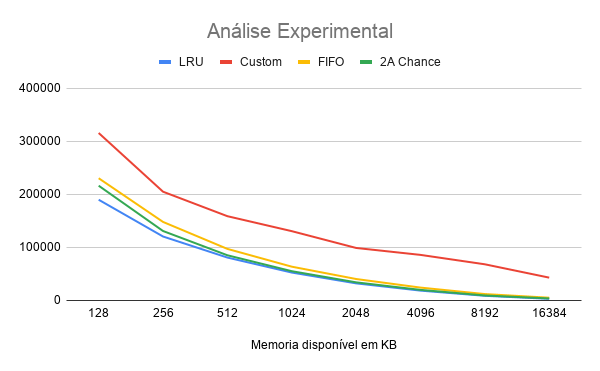
\includegraphics[scale=0.5]{Figuras/img1.png}
% 	\end{center}
% 	\caption{\label{fig:sudoku_grafo_colorido} Transformação do sudoku para grafo colorido.}
% \end{figure}
